\documentclass[tikz,border=2pt]{standalone}
\usepackage{amsmath}
\usepackage{pgfplots}
\pgfplotsset{compat=1.18}

\begin{document}
% Three smoothness levels at 0: |x| is C^0 only (a corner), x|x| is C^1 (its derivative 2|x| has a
% corner), and x^3 is C^∞.
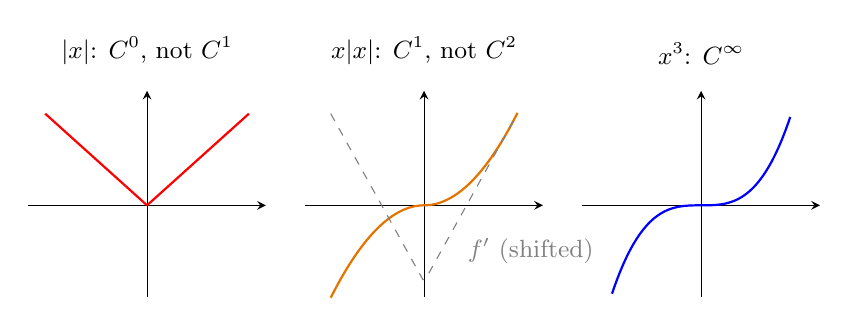
\begin{tikzpicture}
	\begin{axis}[
		name=a,
		axis lines=middle, xmin=-1.4, xmax=1.4, ymin=-1.2, ymax=1.5,
		xtick=\empty, ytick=\empty, samples=80, smooth, clip=false,
		width=4.6cm, height=4.2cm,
		title={$|x|$: $C^0$, not $C^1$}, title style={font=\small}
		]
		\addplot[thick, red, domain=-1.2:0, samples=2] {-x};
		\addplot[thick, red, domain=0:1.2, samples=2] {x};
	\end{axis}
	\begin{axis}[
		name=b, at={(a.east)}, anchor=west, xshift=0.5cm,
		axis lines=middle, xmin=-1.4, xmax=1.4, ymin=-1.2, ymax=1.5,
		xtick=\empty, ytick=\empty, samples=80, smooth, clip=false,
		width=4.6cm, height=4.2cm,
		title={$x|x|$: $C^1$, not $C^2$}, title style={font=\small}
		]
		\addplot[thick, orange!90!black, domain=-1.1:1.1] {x*abs(x)};
		\addplot[gray, dashed, domain=-1.1:1.1] {2*abs(x)-1.0};
		\node[gray, anchor=west, font=\small] at (axis cs:0.4,-0.6) {$f'$ (shifted)};
	\end{axis}
	\begin{axis}[
		at={(b.east)}, anchor=west, xshift=0.5cm,
		axis lines=middle, xmin=-1.4, xmax=1.4, ymin=-1.2, ymax=1.5,
		xtick=\empty, ytick=\empty, samples=80, smooth, clip=false,
		width=4.6cm, height=4.2cm,
		title={$x^3$: $C^\infty$}, title style={font=\small}
		]
		\addplot[thick, blue, domain=-1.05:1.05] {x^3};
	\end{axis}
\end{tikzpicture}
\end{document}
